\chapter*{Zeitmanagement}
	\documentPartEntry{Zeitmanagement}
	%TODO: Kapitel und Bild unten mit den letzten Erkenntnissen und erfassten Zeiten nochmals überarbeiten!
	Für die zeitliche Planung und für die Auswertung der Arbeitszeit haben wir das \ppt\ Jira\footnote{\url{https://de.atlassian.com/software/jira}} verwendet,
	wie wir es auch für das ganze Projektmanagement verwendet haben.
	Wann immer wir einen Task erstellten, haben wir auch die dafür benötigte Dauer geschätzt
	und diese im Jira eingetragen.
	Und auch jede geleistete Arbeit haben wir im Jira erfasst.
	Ein Beispiel für eine Erfassung von Arbeitszeit ist in Abbildung\ \ref{fig:logWork} abgebildet.
	\begin{figure}[H]
		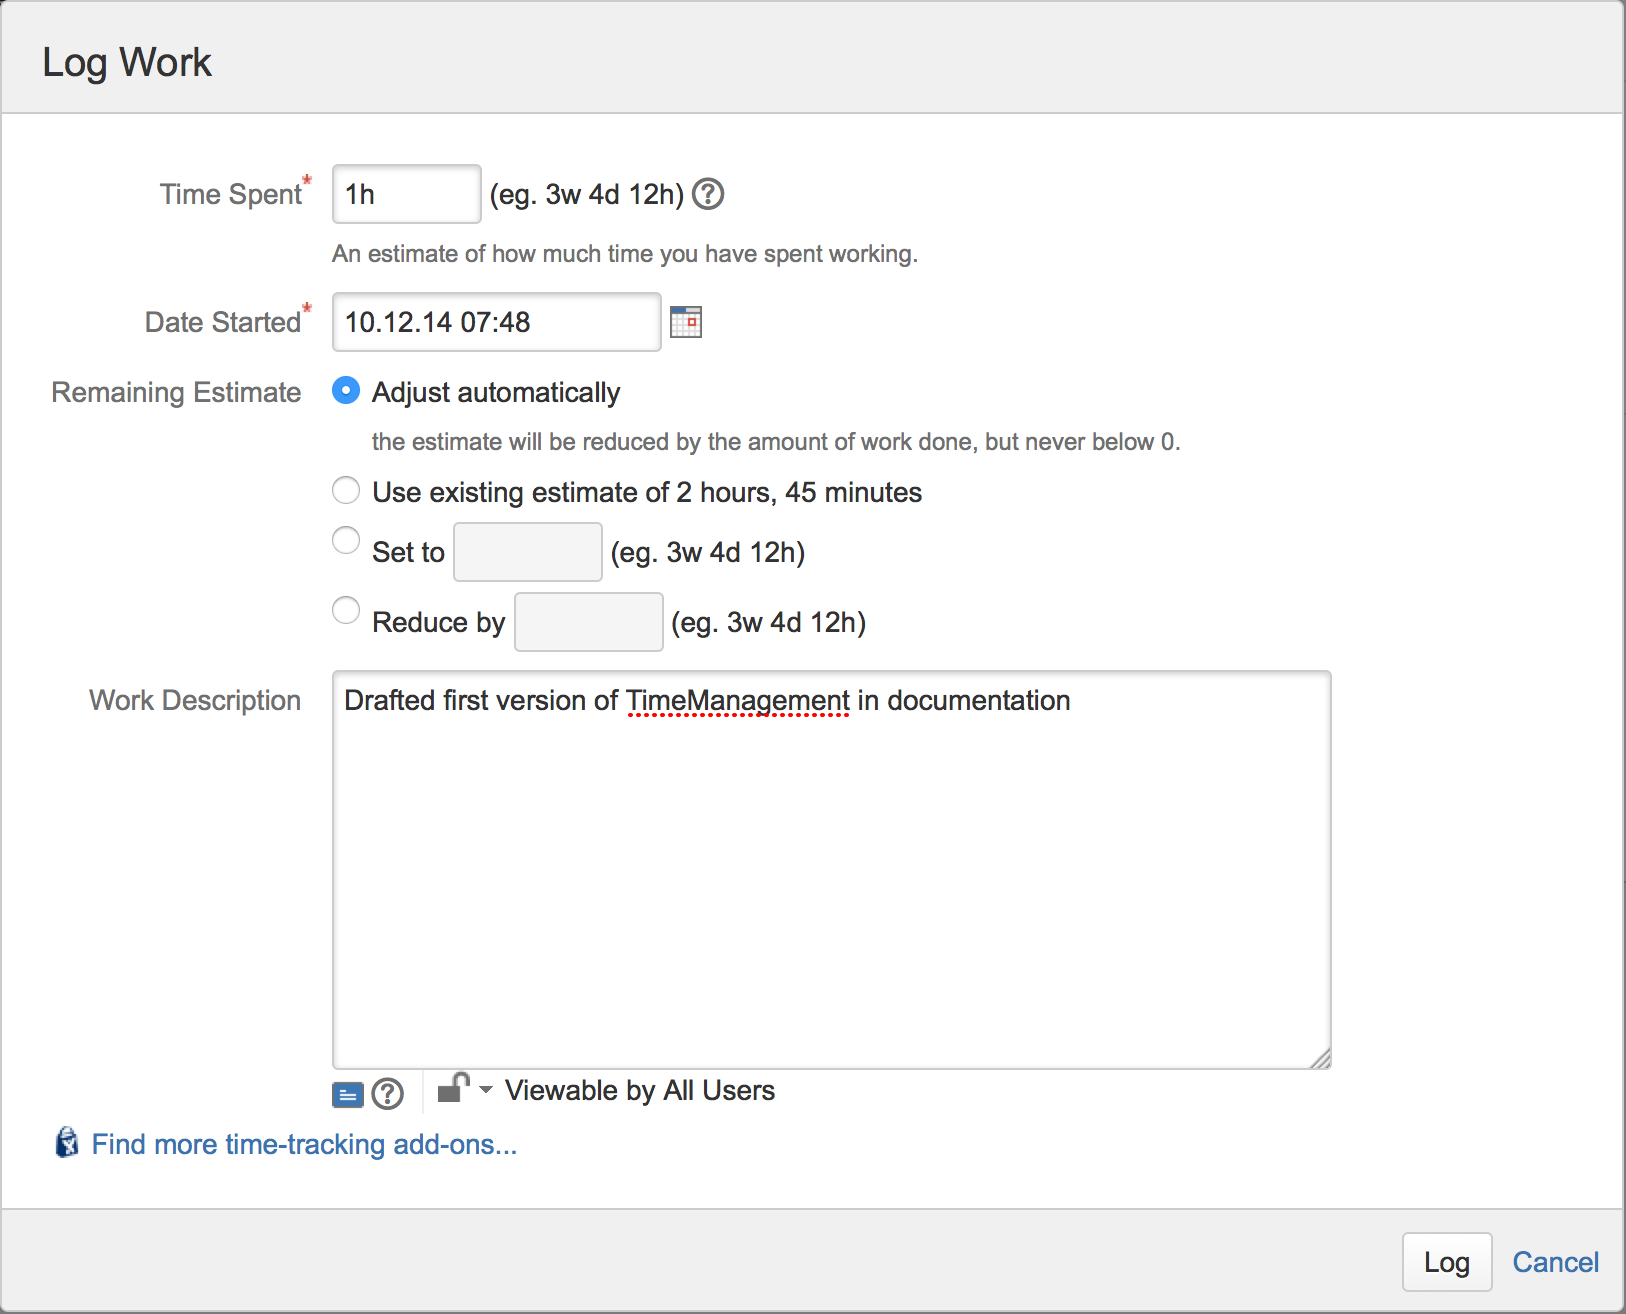
\includegraphics[width=0.5\textwidth]{projectPlan/media/img/logWork.png}
		\centering
		\caption{Erfassen von Arbeitszeit im Jira}
		\label{fig:logWork}
	\end{figure}
	
	Die erfassten Arbeitszeiten haben wir mit einem eigenen Ruby-Skript über die REST API von Jira\footnote{\url{https://docs.atlassian.com/jira/REST/latest/}} exportiert
	und in einer Excel-Tabelle jeweils laufend während dem Projekt ausgewertet.
	Entstanden ist der Graph über die geleistete Arbeit in Abbildung\ \ref{fig:workGraph}.
	Darin sieht man den kontinuierlichen Verlauf während dem Projekt
	und die ausgeglichene Arbeitslast zwischen Tobias Blaser und Laurin Murer.
	Das Ziel war, die Arbeit eine Woche vorher fertig zu haben.
	Deshalb geht auch das maximale Soll nur bis dann.
	Die beiden Soll-Linien geben die von der HSR vorgegebene minimal und maximal erwartete Arbeitszeit an,
	wir waren jeweils immer um das obere Limit.
	\begin{figure}[H]
		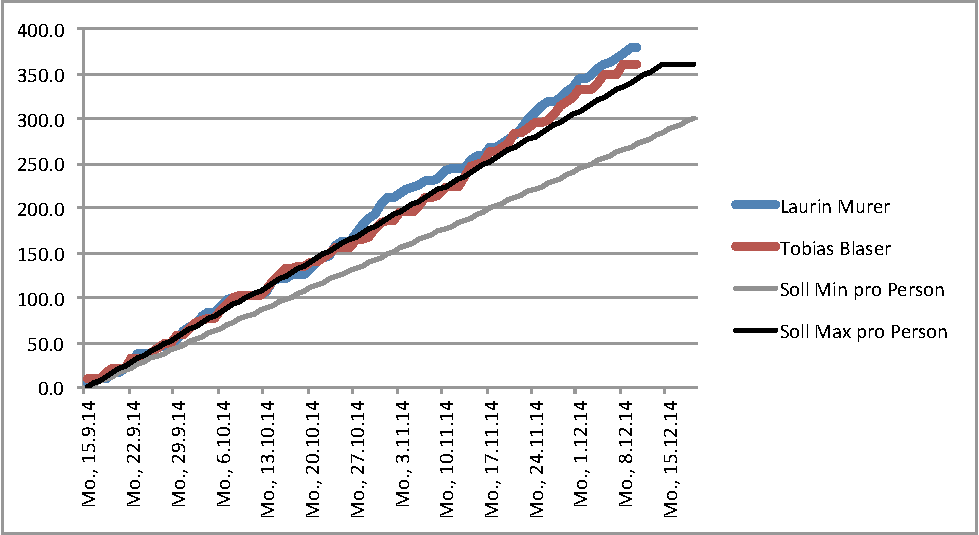
\includegraphics[width=\textwidth]{projectPlan/media/img/workGraph.pdf}
		\centering
		\caption{Graph über die geleistete Arbeit}
		\label{fig:workGraph}
	\end{figure}

%TODO: evtl. Schätzgenauigkeit der Issues auch noch dokumentieren.
